(make use of HW2 and HW3) - (5 points)

Keep your documentation short and to the point. If you are using a framework, you don't need to describe the framework in detail. Instead focus on the big picture. For instance, if you are using a web framework, then you should just explain the metaphor behind it (eg., "Web Framework X is based on the Model-View-Controller pattern. Our models follow the Active Record pattern to interface with the database. ...").

\begin{enumerate}
	\item Include multiple UML diagrams to show the important parts of your system (you must have UML diagrams).
	\item Describe in a top-down manner the architecture of your system.
	\item Include enough details about the design of your system such that anyone who refers to your documentation can understand the major components of your system and how they are related.
	\item Describe how the choice of the framework influence the design of your system.
\end{enumerate}

Check out Figure \ref{us1_sequence}!!

\renewcommand\listfigurename{List of Diagrams}
\listoffigures

\subsection{Expiration Picker}
\begin{figure}[H]
    \centering
    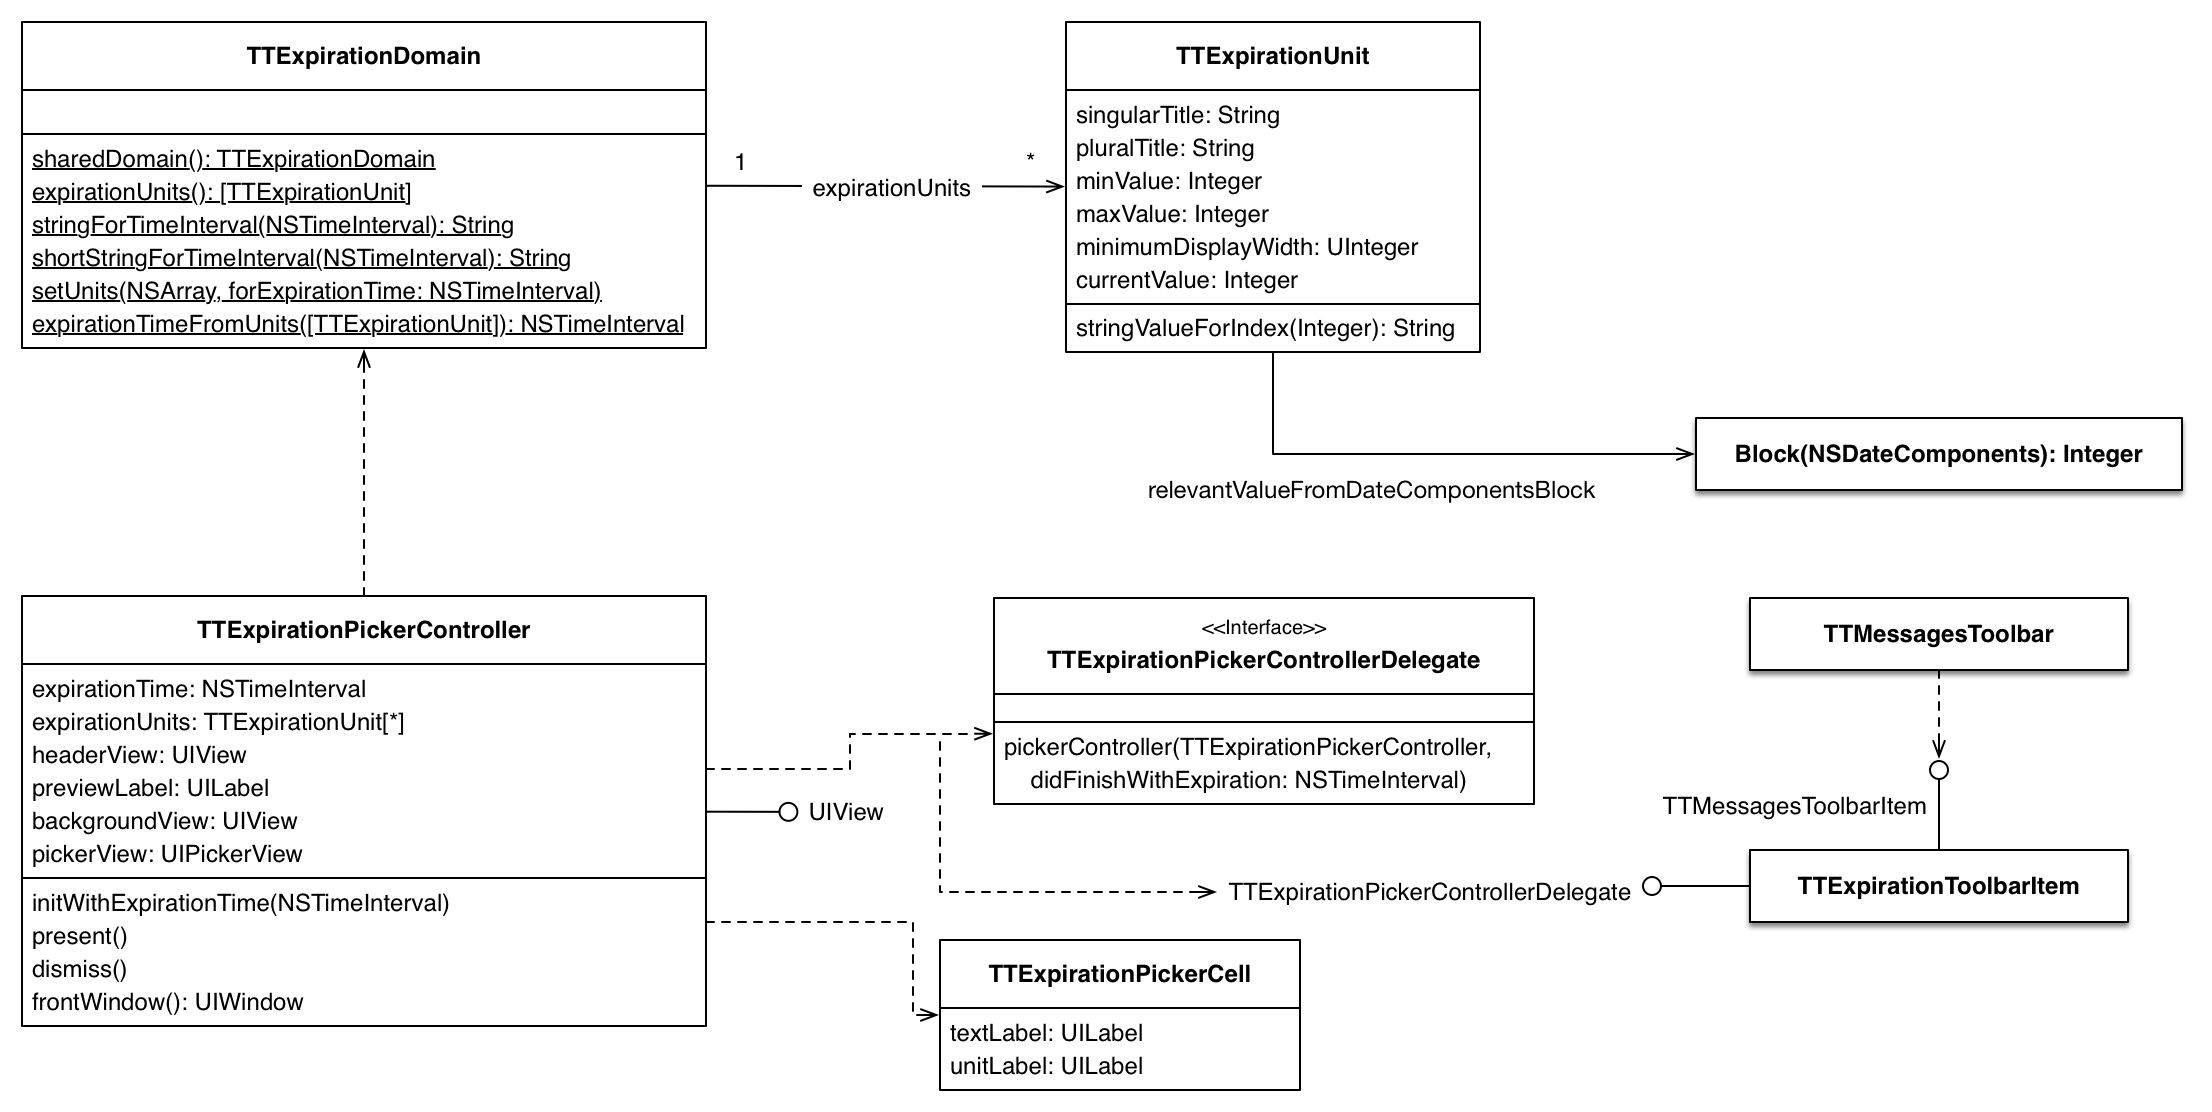
\includegraphics[width=\textwidth]{expirationpicker_class}
    \caption{Expiration Picker Class Diagram}
    \label{fig:expirationpicker_classdiagram}
\end{figure}

\begin{figure}[H]
    \centering
    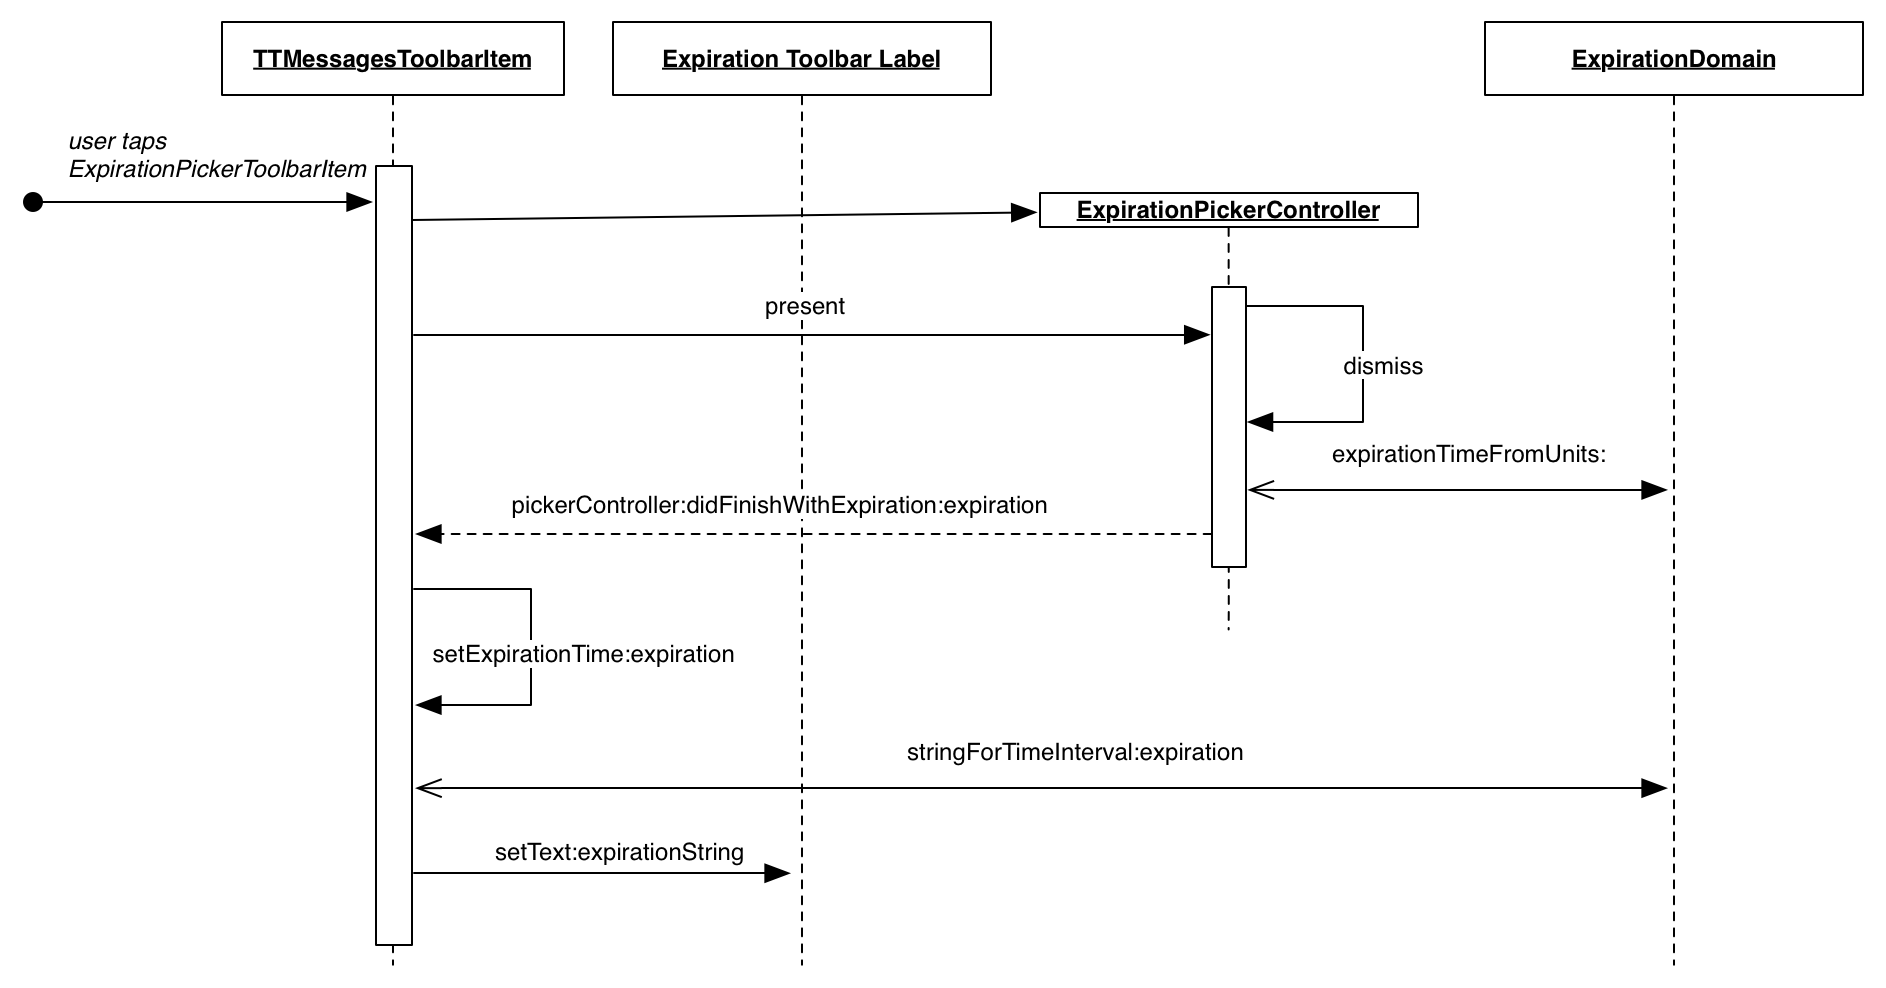
\includegraphics[width=\textwidth]{expirationpicker_sequence}
    \caption{Expiration Picker Sequence Diagram}
    \label{fig:expirationpicker_sequence}
\end{figure}

\subsection{Sequence Diagrams}
\begin{figure}[H]
    \centering
    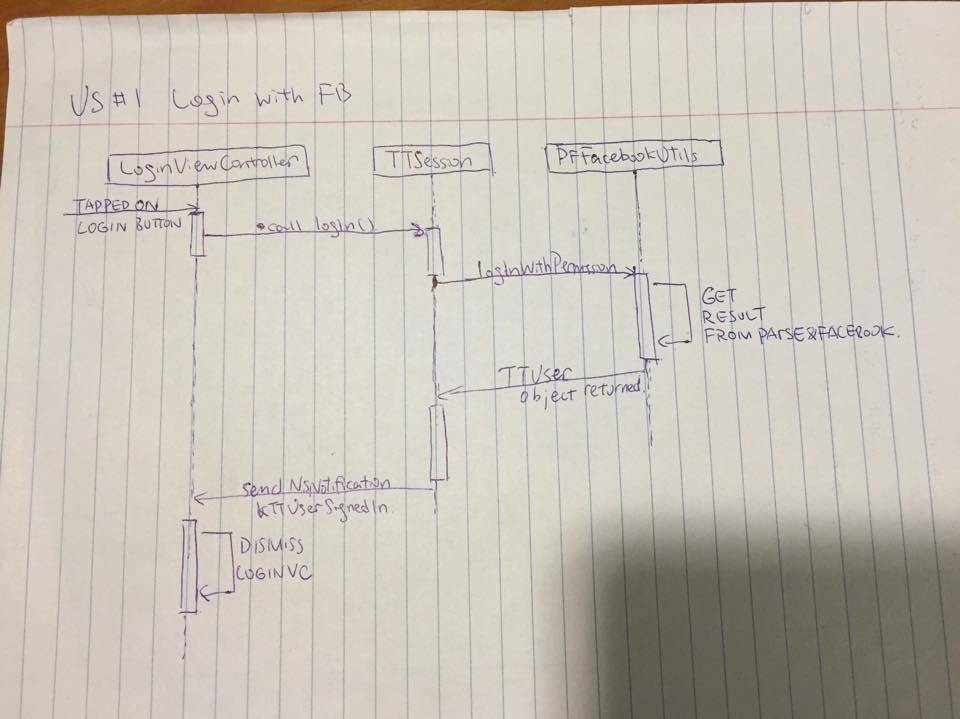
\includegraphics[width=0.8\textwidth]{us1_sequence}
    \caption{US1 Sequence Diagram}
    \label{fig:us1_sequence}
\end{figure}

\begin{figure}[H]
    \centering
    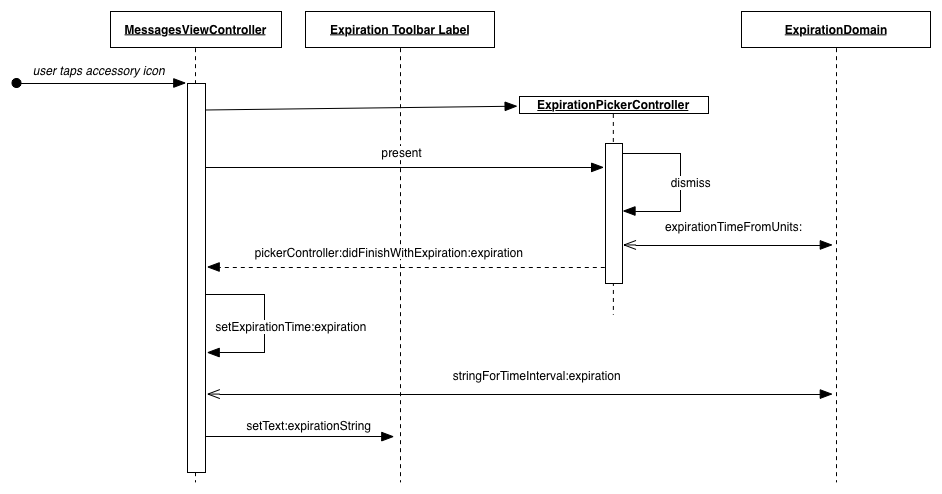
\includegraphics[width=0.8\textwidth]{us4_sequence}
    \caption{US4 Sequence Diagram}
    \label{fig:us4_sequence}
\end{figure}

\begin{figure}[H]
    \centering
    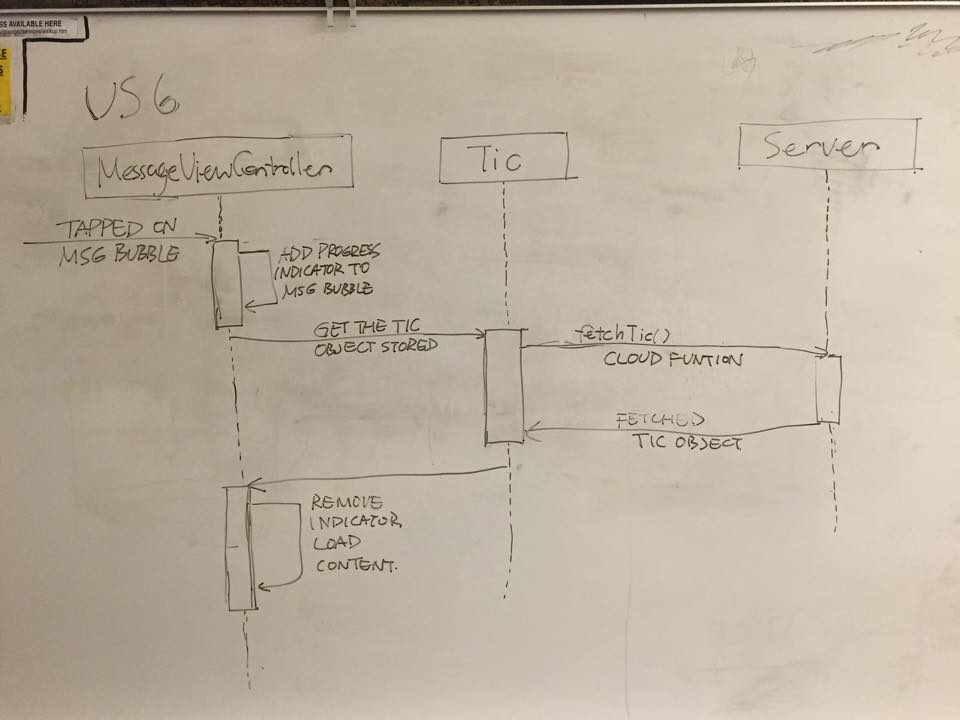
\includegraphics[width=0.8\textwidth]{us6_sequence}
    \caption{US6 Sequence Diagram}
    \label{fig:us6_sequence}
\end{figure}

\begin{figure}[H]
    \centering
    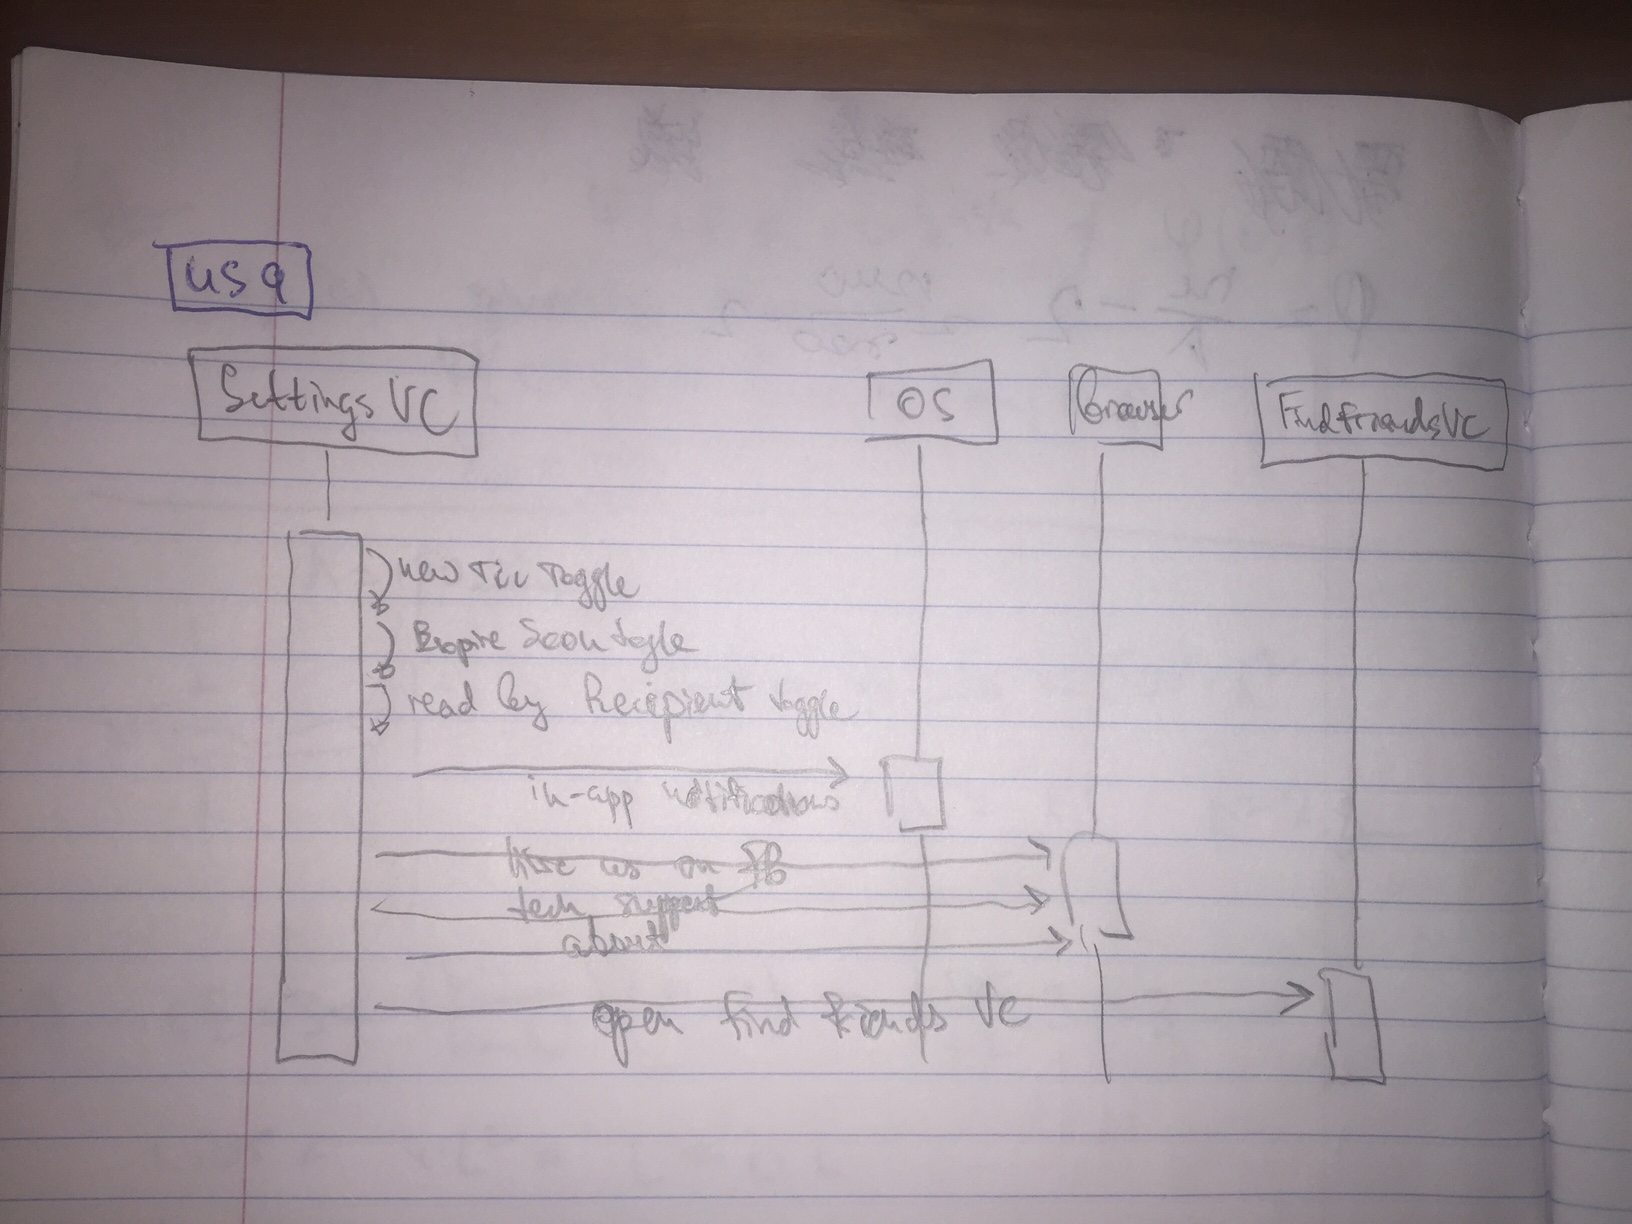
\includegraphics[width=0.8\textwidth]{us9_sequence}
    \caption{US9 Sequence Diagram}
    \label{fig:us9_sequence}
\end{figure}

\begin{figure}[H]
    \centering
    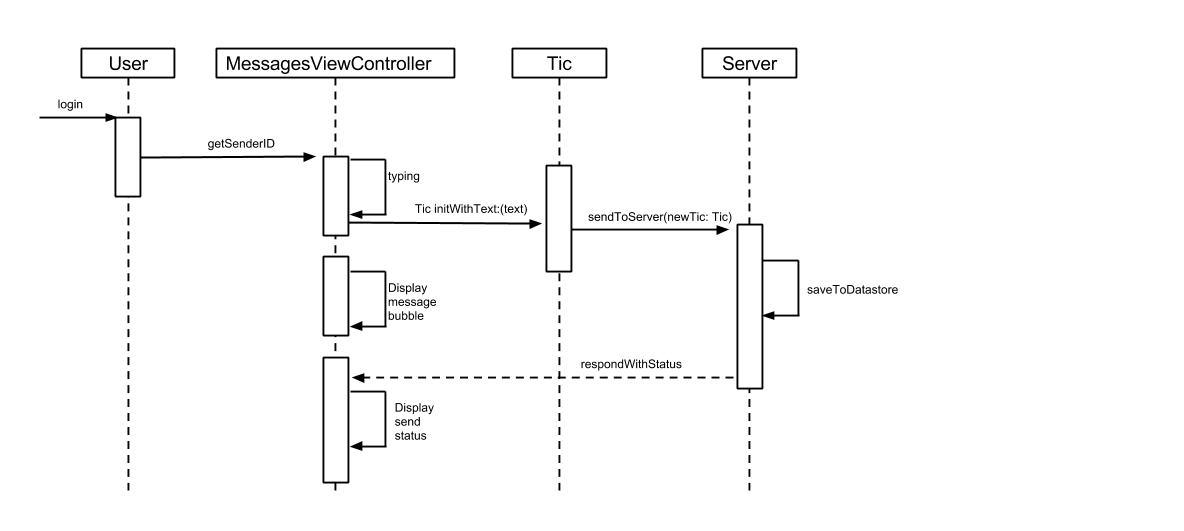
\includegraphics[width=0.8\textwidth]{us11_sequence}
    \caption{US11 Sequence Diagram}
    \label{fig:us11_sequence}
\end{figure}

\begin{figure}[H]
    \centering
    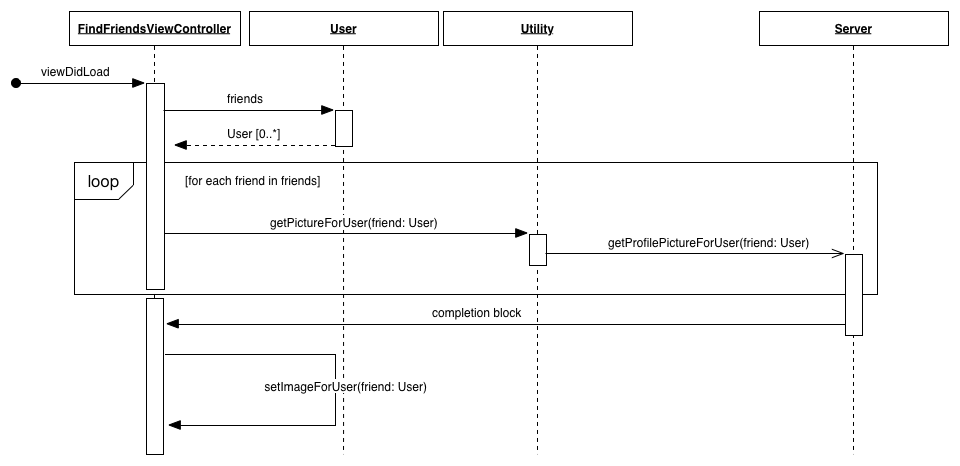
\includegraphics[width=0.8\textwidth]{us15_sequence}
    \caption{US15 Sequence Diagram}
    \label{fig:us15_sequence}
\end{figure}
